\documentclass{article}
\usepackage{tikz}
\usepackage{comment}
\usetikzlibrary{positioning}

\pgfdeclarelayer{bg}    % declare background layer
\pgfsetlayers{bg,main}  % set the order of the layers (main is the standard layer)

\begin{document}
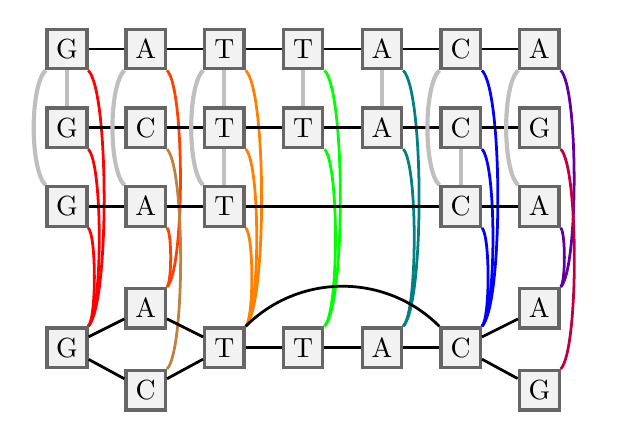
\begin{tikzpicture}[auto,
    node distance= 10mm and 20mm,
    roundnode/.style={circle, draw=black!60, fill=gray!10, very thick, minimum size=7mm},
    squarednode/.style={rectangle, draw=black!60, fill=gray!10, very thick, minimum size=5mm},
    keynode/.style={rectangle, draw=black!60, fill=gray!10, thick, minimum size=1mm}
]
%Nodes
\node[squarednode] (seqA1) {G};
\node[squarednode] (seqA2) [right of=seqA1] {A};
\node[squarednode] (seqA3) [right of=seqA2] {T};
\node[squarednode] (seqA4) [right of=seqA3] {T};
\node[squarednode] (seqA5) [right of=seqA4] {A};
\node[squarednode] (seqA6) [right of=seqA5] {C};
\node[squarednode] (seqA7) [right of=seqA6] {A};

\node[squarednode] (seqB1) [below of=seqA1] {G};
\node[squarednode] (seqB2) [right of=seqB1] {C};
\node[squarednode] (seqB3) [right of=seqB2] {T};
\node[squarednode] (seqB4) [right of=seqB3] {T};
\node[squarednode] (seqB5) [right of=seqB4] {A};
\node[squarednode] (seqB6) [right of=seqB5] {C};
\node[squarednode] (seqB7) [right of=seqB6] {G};

\node[squarednode] (seqC1) [below of=seqB1] {G};
\node[squarednode] (seqC2) [right of=seqC1] {A};
\node[squarednode] (seqC3) [right of=seqC2] {T};
\node[squarednode] (seqC4) [below of=seqB6] {C};
\node[squarednode] (seqC5) [right of=seqC4] {A};

%Lines
\draw[line width=1.0] (seqA1) -- (seqA2);
\draw[line width=1.0] (seqA2) -- (seqA3);
\draw[line width=1.0] (seqA3) -- (seqA4);
\draw[line width=1.0] (seqA4) -- (seqA5);
\draw[line width=1.0] (seqA5) -- (seqA6);
\draw[line width=1.0] (seqA6) -- (seqA7);

\draw[line width=1.0] (seqB1) -- (seqB2);
\draw[line width=1.0] (seqB2) -- (seqB3);
\draw[line width=1.0] (seqB3) -- (seqB4);
\draw[line width=1.0] (seqB4) -- (seqB5);
\draw[line width=1.0] (seqB5) -- (seqB6);
\draw[line width=1.0] (seqB6) -- (seqB7);

\draw[line width=1.0] (seqC1) -- (seqC2);
\draw[line width=1.0] (seqC2) -- (seqC3);
\draw[line width=1.0] (seqC3) -- (seqC4);
\draw[line width=1.0] (seqC4) -- (seqC5);

% alignments
\draw[line width=1.5,color=gray!50] (seqA1) -- (seqB1);
\draw[line width=1.5,color=gray!50] (seqA1) to [in=135,out=225,looseness=0.5, edge node={node [sloped,above] {}}] (seqC1);
%\draw[line width=1.0,color=gray!100] (seqA2) -- (seqB2);
\draw[line width=1.5,color=gray!50] (seqA2) to [in=135,out=225,looseness=0.5, edge node={node [sloped,above] {}}] (seqC2);

\draw[line width=1.5,color=gray!50] (seqA3) -- (seqB3);
\draw[line width=1.5,color=gray!50] (seqA3) to [in=135,out=225,looseness=0.5, edge node={node [sloped,above] {}}] (seqC3);
\draw[line width=1.5,color=gray!50] (seqB3) -- (seqC3);

\draw[line width=1.5,color=gray!50] (seqA4) -- (seqB4);
\draw[line width=1.5,color=gray!50] (seqA5) -- (seqB5);

%\draw[line width=1.5,color=gray!50] (seqA6) -- (seqB6);
\draw[line width=1.5,color=gray!50] (seqA6) to [in=135,out=225,looseness=0.5, edge node={node [sloped,above] {}}] (seqC4);
\draw[line width=1.5,color=gray!50] (seqB6) -- (seqC4);

%\draw[line width=1.5,color=gray!50] (seqA7) -- (seqB7);
\draw[line width=1.5,color=gray!50] (seqA7) to [in=135,out=225,looseness=0.5, edge node={node [sloped,above] {}}] (seqC5);
%\draw[line width=1.5,color=gray!50] (seqB7) -- (seqC5);


%    \draw (i) to[out=150, in=210, looseness=4, edge node={node [sloped,below] {$\leftarrow$}}] (l);
%    \draw (k) to[out=30, in=-30, looseness=4, edge node={node [sloped,above] {$\leftarrow$}}] (j);

%\begin{scope}[node distance=1cm]
\node[squarednode] (g2) [below = 0.75cm of seqC2] {A};
\node[squarednode] (g1) [below = 1.25cm of seqC1] {G};
\node[squarednode] (g3) [below = 0.5cm of g2] {C};
\node[squarednode] (g4) [below = 1.25cm of seqC3] {T};
\node[squarednode] (g5) [right of=g4] {T};
\node[squarednode] (g6) [right of=g5] {A};
\node[squarednode] (g7) [below = 1.25cm of seqC4] {C};
\node[squarednode] (g8) [below = 0.75cm of seqC5] {A};
\node[squarednode] (g9) [below = 0.5cm of g8] {G};
%\end{scope}

\draw[line width=1.0] (g1) to (g2);
\draw[line width=1.0] (g1) to (g3);
\draw[line width=1.0] (g2) to (g4);
\draw[line width=1.0] (g3) to (g4);
\draw[line width=1.0] (g4) to (g5);
\draw[line width=1.0] (g4) to [looseness=1] (g7);
\draw[line width=1.0] (g5) to (g6);
\draw[line width=1.0] (g6) to (g7);
\draw[line width=1.0] (g7) to (g8);
\draw[line width=1.0] (g7) to (g9);

\begin{pgfonlayer}{bg}    % select the background layer
\draw[line width=1.0,color=red!100] (seqA1) to [looseness=0.3,in=45,out=-45, edge node={node [sloped,above] {}}] (g1);
\draw[line width=1.0,color=red!100] (seqB1) to [looseness=0.3,in=45,out=-45, edge node={node [sloped,above] {}}] (g1);
\draw[line width=1.0,color=red!100] (seqC1) to [looseness=0.3,in=45,out=-45, edge node={node [sloped,above] {}}] (g1);
%\draw[line width=1.0,color=red!100,looseness=0.5] (seqB1.south) to (g1.north);
%\draw[line width=1.0,color=red!100,looseness=0.5] (seqC1.south) to (g1.north);

\draw[line width=1.0,color={rgb:red,1;orange,1}] (seqA2) to [looseness=0.3,in=45,out=-45, edge node={node [sloped,above] {}}] (g2);
\draw[line width=1.0,color={rgb:red,1;orange,1}] (seqC2) to [looseness=0.3,in=45,out=-45, edge node={node [sloped,above] {}}] (g2);

\draw[line width=1.0,color=orange!100] (seqA3) to [looseness=0.3,in=45,out=-45, edge node={node [sloped,above] {}}] (g4);
\draw[line width=1.0,color=orange!100] (seqB3) to [looseness=0.3,in=45,out=-45, edge node={node [sloped,above] {}}] (g4);
\draw[line width=1.0,color=orange!100] (seqC3) to [looseness=0.3,in=45,out=-45, edge node={node [sloped,above] {}}] (g4);

\draw[line width=1.0,color=green!100] (seqA4) to [looseness=0.3,in=45,out=-45, edge node={node [sloped,above] {}}] (g5);
\draw[line width=1.0,color=green!100] (seqB4) to [looseness=0.3,in=45,out=-45, edge node={node [sloped,above] {}}] (g5);
%\draw[line width=1.0,color=blue!100] (seqC3) to [looseness=0.3,in=45,out=-45, edge node={node [sloped,above] {}}] (g4);

\draw[line width=1.0,color={rgb:blue,1;green,1}] (seqA5) to [looseness=0.3,in=45,out=-45, edge node={node [sloped,above] {}}] (g6);
\draw[line width=1.0,color={rgb:blue,1;green,1}] (seqB5) to [looseness=0.3,in=45,out=-45, edge node={node [sloped,above] {}}] (g6);

\draw[line width=1.0,color=blue!100] (seqA6) to [looseness=0.3,in=45,out=-45, edge node={node [sloped,above] {}}] (g7);
\draw[line width=1.0,color=blue!100] (seqB6) to [looseness=0.3,in=45,out=-45, edge node={node [sloped,above] {}}] (g7);
\draw[line width=1.0,color=blue!100] (seqC4) to [looseness=0.3,in=45,out=-45, edge node={node [sloped,above] {}}] (g7);

\draw[line width=1.0,color={rgb:blue,1;purple,1}] (seqA7) to [looseness=0.3,in=45,out=-45, edge node={node [sloped,above] {}}] (g8);
\draw[line width=1.0,color={rgb:blue,1;purple,1}] (seqC5) to [looseness=0.3,in=45,out=-45, edge node={node [sloped,above] {}}] (g8);

\draw[line width=1.0,color=purple!100] (seqB7) to [looseness=0.3,in=45,out=-45, edge node={node [sloped,above] {}}] (g9);

\draw[line width=1.0,color=brown] (seqB2) to [looseness=0.3,in=45,out=-45, edge node={node [sloped,above] {}}] (g3);

\begin{comment}
\begin{scope}[node distance=0.5cm]
  \node[keynode,fill=red!100] (c1) [right = 1cm of seqA7] {1};
  \node[keynode,fill={rgb:red,1;orange,1}] (c2) [below of=c1] {2};
  \node[keynode,fill=orange!100] (c3) [below of=c2] {3};
  \node[keynode,fill=green!100] (c4) [below of=c3] {4};
  \node[keynode,fill={rgb:blue,1;green,1},text=white] (c5) [below of=c4] {5};
  \node[keynode,fill=blue!100,text=white] (c6) [below of=c5] {6};
  \node[keynode,fill={rgb:blue,1;purple,1},text=white] (c7) [below of=c6] {7};
  \node[keynode,fill=purple!100] (c8) [below of=c7] {8};
  \node[keynode,fill=gray] (c9) [below of=c8] {9};
\end{scope}
\end{comment}

\end{pgfonlayer}

%\draw[->] (uppercircle.south) -- (seq1.north);
%\draw[->] (seq1.east) -- (rightsquare.west);
%\draw[->] (rightsquare.south) .. controls +(down:7mm) and +(right:7mm) .. (lowercircle.east);
%\draw[->] (rightsquare.south) -- (lowercircle.east);
\end{tikzpicture}
\end{document}
